\chapter{Thiết kế hệ thống}

\section{Giới thiệu}
Chương này trình bày các kết quả thiết kế hệ thống dựa trên phân tích ở Chương 2, bao gồm: thiết kế cơ sở dữ liệu, thiết kế kiến trúc, thiết kế giao diện và thiết kế API. Đây là nền tảng để triển khai cài đặt ở Chương tiếp theo.

\section{Thiết kế cơ sở dữ liệu}

\subsection{Mô hình thực thể - quan hệ (ER Diagram)}
Hệ thống sử dụng MongoDB, do đó mô hình được thiết kế dưới dạng các collection. Hình \ref{fig:erd} mô tả mối quan hệ giữa các thực thể chính.

\begin{figure}[H]
\centering
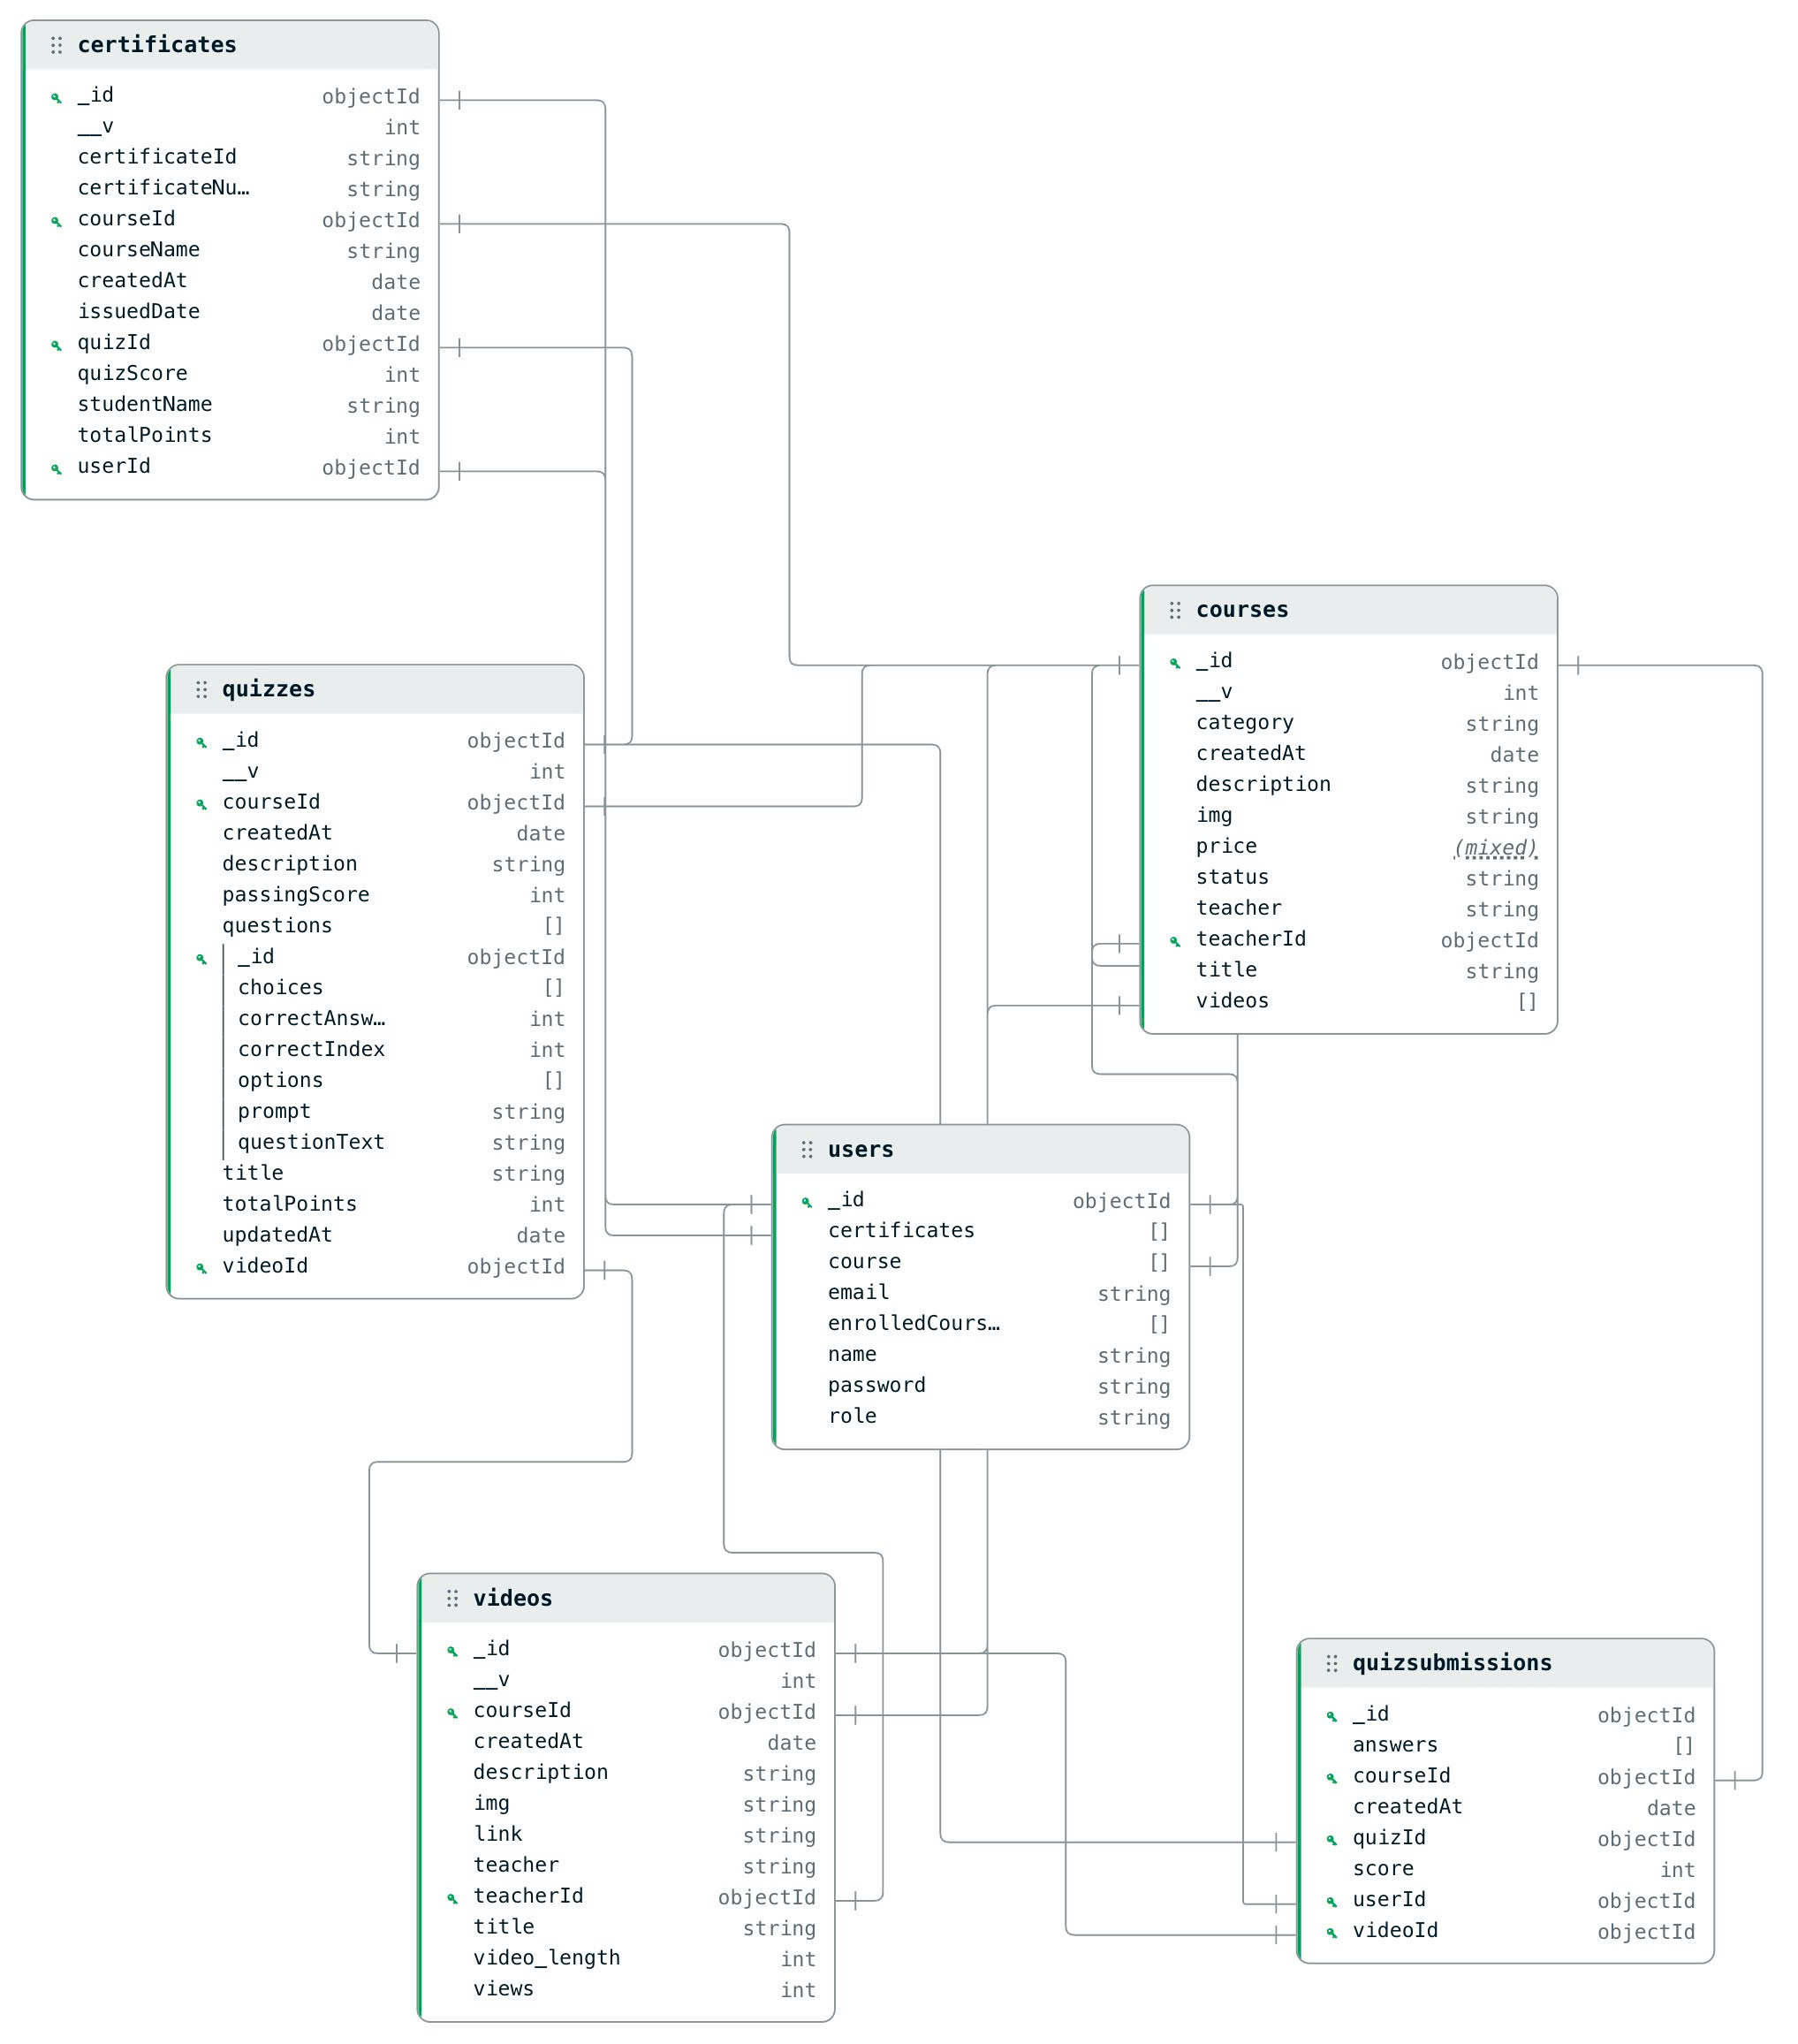
\includegraphics[width=0.9\textwidth]{figs/erd.jpg}
\caption{Sơ đồ ERD của hệ thống}
\label{fig:erd}
\end{figure}

\subsection{Mô tả các collection}
Hệ thống sử dụng MongoDB với các collection chính được thiết kế dựa trên ERD. Dưới đây là mô tả chi tiết từng collection.

\begin{table}[H]
\centering
\caption{Collection Users}
\begin{tabular}{|p{2.5cm}|p{2.5cm}|p{2.5cm}|p{5cm}|}
\hline
\textbf{Trường} & \textbf{Kiểu} & \textbf{Ràng buộc} & \textbf{Mô tả} \\ \hline
\_id & ObjectId & PK & Khóa chính \\ \hline
name & String & NOT NULL & Họ tên người dùng \\ \hline
email & String & UNIQUE, NOT NULL & Email đăng nhập \\ \hline
password & String & NOT NULL & Mật khẩu đã được bcrypt \\ \hline
role & String & 'admin','teacher','student' & Vai trò trong hệ thống \\ \hline
certificates & Array & - & Danh sách chứng chỉ đã đạt (tham chiếu) \\ \hline
course & Array & - & Khóa học đã tạo (nếu là teacher) \\ \hline
enrolledCourses & Array & - & Danh sách khóa học đã ghi danh \\ \hline
\end{tabular}
\end{table}

\begin{table}[H]
\centering
\caption{Collection Courses}
\begin{tabular}{|p{2.5cm}|p{2.5cm}|p{2.5cm}|p{5cm}|}
\hline
\textbf{Trường} & \textbf{Kiểu} & \textbf{Ràng buộc} & \textbf{Mô tả} \\ \hline
\_id & ObjectId & PK & Khóa chính \\ \hline
title & String & NOT NULL & Tên khóa học \\ \hline
description & String & - & Mô tả chi tiết khóa học \\ \hline
category & String & - & Danh mục (ví dụ: Lập trình, Ngoại ngữ) \\ \hline
price & Mixed & - & Giá khóa học (có thể là số hoặc chuỗi) \\ \hline
img & String & - & URL ảnh đại diện khóa học \\ \hline
status & String & 'public','draft' & Trạng thái hiển thị \\ \hline
teacher & String & - & Tên giảng viên \\ \hline
teacherId & ObjectId & FK -> Users.\_id & ID giảng viên tạo khóa học \\ \hline
createdAt & Date & DEFAULT NOW & Thời gian tạo \\ \hline
videos & Array & - & Danh sách video (có thể nhúng) \\ \hline
\end{tabular}
\end{table}

\begin{table}[H]
\centering
\caption{Collection Videos}
\begin{tabular}{|p{2.5cm}|p{2.5cm}|p{2.5cm}|p{5cm}|}
\hline
\textbf{Trường} & \textbf{Kiểu} & \textbf{Ràng buộc} & \textbf{Mô tả} \\ \hline
\_id & ObjectId & PK & Khóa chính \\ \hline
title & String & NOT NULL & Tiêu đề video \\ \hline
description & String & - & Mô tả video \\ \hline
link & String & NOT NULL & URL video (Cloudinary) \\ \hline
img & String & - & URL ảnh thumbnail \\ \hline
video\_length & Number & - & Thời lượng (giây hoặc phút) \\ \hline
views & Number & DEFAULT 0 & Số lượt xem \\ \hline
courseId & ObjectId & FK -> Courses.\_id & Khóa học chứa video \\ \hline
teacher & String & - & Tên giảng viên \\ \hline
teacherId & ObjectId & FK -> Users.\_id & ID giảng viên upload \\ \hline
createdAt & Date & DEFAULT NOW & Ngày tạo \\ \hline
\end{tabular}
\end{table}

\begin{table}[H]
\centering
\caption{Collection Quizzes}
\begin{tabular}{|p{2.5cm}|p{2.5cm}|p{2.5cm}|p{5cm}|}
\hline
\textbf{Trường} & \textbf{Kiểu} & \textbf{Ràng buộc} & \textbf{Mô tả} \\ \hline
\_id & ObjectId & PK & Khóa chính \\ \hline
title & String & NOT NULL & Tiêu đề bộ câu hỏi \\ \hline
description & String & - & Mô tả quiz \\ \hline
questions & Array & NOT NULL & Danh sách câu hỏi (mỗi câu có prompt, options, correctAnswer, ...) \\ \hline
passingScore & Number & 0-100 & Điểm cần đạt để vượt qua \\ \hline
totalPoints & Number & NOT NULL & Tổng điểm tối đa \\ \hline
courseId & ObjectId & FK -> Courses.\_id & Khóa học chứa quiz \\ \hline
videoId & ObjectId & FK -> Videos.\_id & Video liên quan (nếu có) \\ \hline
createdAt & Date & DEFAULT NOW & Ngày tạo \\ \hline
updatedAt & Date & - & Ngày cập nhật gần nhất \\ \hline
\end{tabular}
\end{table}

\begin{table}[H]
\centering
\caption{Collection QuizSubmissions}
\begin{tabular}{|p{2.5cm}|p{2.5cm}|p{2.5cm}|p{5cm}|}
\hline
\textbf{Trường} & \textbf{Kiểu} & \textbf{Ràng buộc} & \textbf{Mô tả} \\ \hline
\_id & ObjectId & PK & Khóa chính \\ \hline
answers & Array & NOT NULL & Mảng câu trả lời của học viên \\ \hline
score & Number & 0-100 & Điểm đạt được \\ \hline
userId & ObjectId & FK -> Users.\_id & Học viên làm bài \\ \hline
quizId & ObjectId & FK -> Quizzes.\_id & Quiz tương ứng \\ \hline
courseId & ObjectId & FK -> Courses.\_id & Khóa học \\ \hline
videoId & ObjectId & FK -> Videos.\_id & Video liên quan (nếu có) \\ \hline
createdAt & Date & DEFAULT NOW & Thời gian nộp bài \\ \hline
\end{tabular}
\end{table}

\begin{table}[H]
\centering
\caption{Collection Certificates}
\begin{tabular}{|p{2.5cm}|p{2.5cm}|p{2.5cm}|p{5cm}|}
\hline
\textbf{Trường} & \textbf{Kiểu} & \textbf{Ràng buộc} & \textbf{Mô tả} \\ \hline
\_id & ObjectId & PK & Khóa chính \\ \hline
certificateId & String & UNIQUE & Mã chứng chỉ duy nhất \\ \hline
certificateNumber & String & - & Số hiệu chứng chỉ \\ \hline
studentName & String & NOT NULL & Tên học viên \\ \hline
userId & ObjectId & FK -> Users.\_id & Học viên sở hữu \\ \hline
courseId & ObjectId & FK -> Courses.\_id & Khóa học hoàn thành \\ \hline
courseName & String & NOT NULL & Tên khóa học (lưu kèm) \\ \hline
quizId & ObjectId & FK -> Quizzes.\_id & Bài kiểm tra cuối khóa \\ \hline
quizScore & Number & 0-100 & Điểm bài kiểm tra \\ \hline
totalPoints & Number & - & Tổng điểm tối đa của quiz \\ \hline
issuedDate & Date & NOT NULL & Ngày cấp chứng chỉ \\ \hline
createdAt & Date & DEFAULT NOW & Ngày tạo bản ghi \\ \hline
\end{tabular}
\end{table}

\subsection{Ràng buộc toàn vẹn}
Dựa trên phân tích nghiệp vụ và use case, các ràng buộc toàn vẹn sau được áp dụng:
\begin{itemize}
    \item \textbf{Users:} Email là duy nhất. Vai trò chỉ nhận một trong ba giá trị: 'admin', 'teacher', 'student'.
    \item \textbf{Courses:} Một khóa học chỉ có một giảng viên (teacherId), nhưng một giảng viên có thể tạo nhiều khóa học. Khi xóa giảng viên, cần xử lý các khóa học (có thể chuyển sang admin hoặc ẩn).
    \item \textbf{Videos:} Mỗi video thuộc về một khóa học (courseId). Khi xóa khóa học, tất cả video liên quan cũng bị xóa (cascade).
    \item \textbf{Quizzes:} Mỗi quiz thuộc về một khóa học (courseId) và có thể liên kết với một video (videoId). Khi xóa khóa học, các quiz cũng bị xóa.
    \item \textbf{QuizSubmissions:} Mỗi học viên chỉ được nộp bài tối đa một lần cho một quiz (cặp userId + quizId là duy nhất). Điểm số (score) phải nằm trong khoảng 0 đến totalPoints của quiz.
    \item \textbf{Certificates:} Một học viên chỉ được cấp một chứng chỉ cho một khóa học (cặp userId + courseId là duy nhất). Ngày cấp chứng chỉ phải sau ngày hoàn thành khóa học.
    \item \textbf{Quan hệ giữa Users và Courses:} Trong collection Users, trường enrolledCourses lưu danh sách ID các khóa học mà học viên đã ghi danh. Cần đảm bảo tính nhất quán với bảng ghi danh thực tế (có thể dùng trigger ở tầng ứng dụng).
\end{itemize}
\section{Thiết kế kiến trúc}
Hệ thống áp dụng mô hình kiến trúc 3 lớp (three-tier architecture) với MERN Stack:

\begin{figure}[H]
\centering
\begin{tikzpicture}[
    node distance=1.2cm,
    box/.style={rectangle, draw=blue!50, rounded corners, fill=blue!5, minimum width=3.5cm, minimum height=1cm, align=center},
    arrow/.style={-Stealth, thick}
]
\node[box] (client) {\textbf{Tầng giao diện (Client)}\\React.js};
\node[box, below=of client] (server) {\textbf{Tầng logic (Server)}\\Node.js + Express.js};
\node[box, below=of server] (db) {\textbf{Tầng dữ liệu}\\MongoDB};
\draw[arrow] (client) -- (server) node[midway,right] {HTTP/REST};
\draw[arrow] (server) -- (db) node[midway,right] {Mongoose ODM};
\end{tikzpicture}
\caption{Kiến trúc 3 lớp của hệ thống}
\label{fig:architecture}
\end{figure}

Trong đó:
\begin{itemize}
    \item \textbf{Tầng giao diện:} React.js + Redux Toolkit quản lý state, Tailwind CSS cho giao diện responsive.
    \item \textbf{Tầng logic:} Node.js + Express.js cung cấp RESTful API, xác thực JWT, xử lý upload file.
    \item \textbf{Tầng dữ liệu:} MongoDB Atlas lưu trữ, Mongoose làm ODM.
\end{itemize}

\section{Thiết kế giao diện}
Hệ thống có các giao diện chính dành cho từng vai trò. Dưới đây là một số màn hình tiêu biểu (ảnh chụp từ project thực tế).

\begin{figure}[H]
\centering
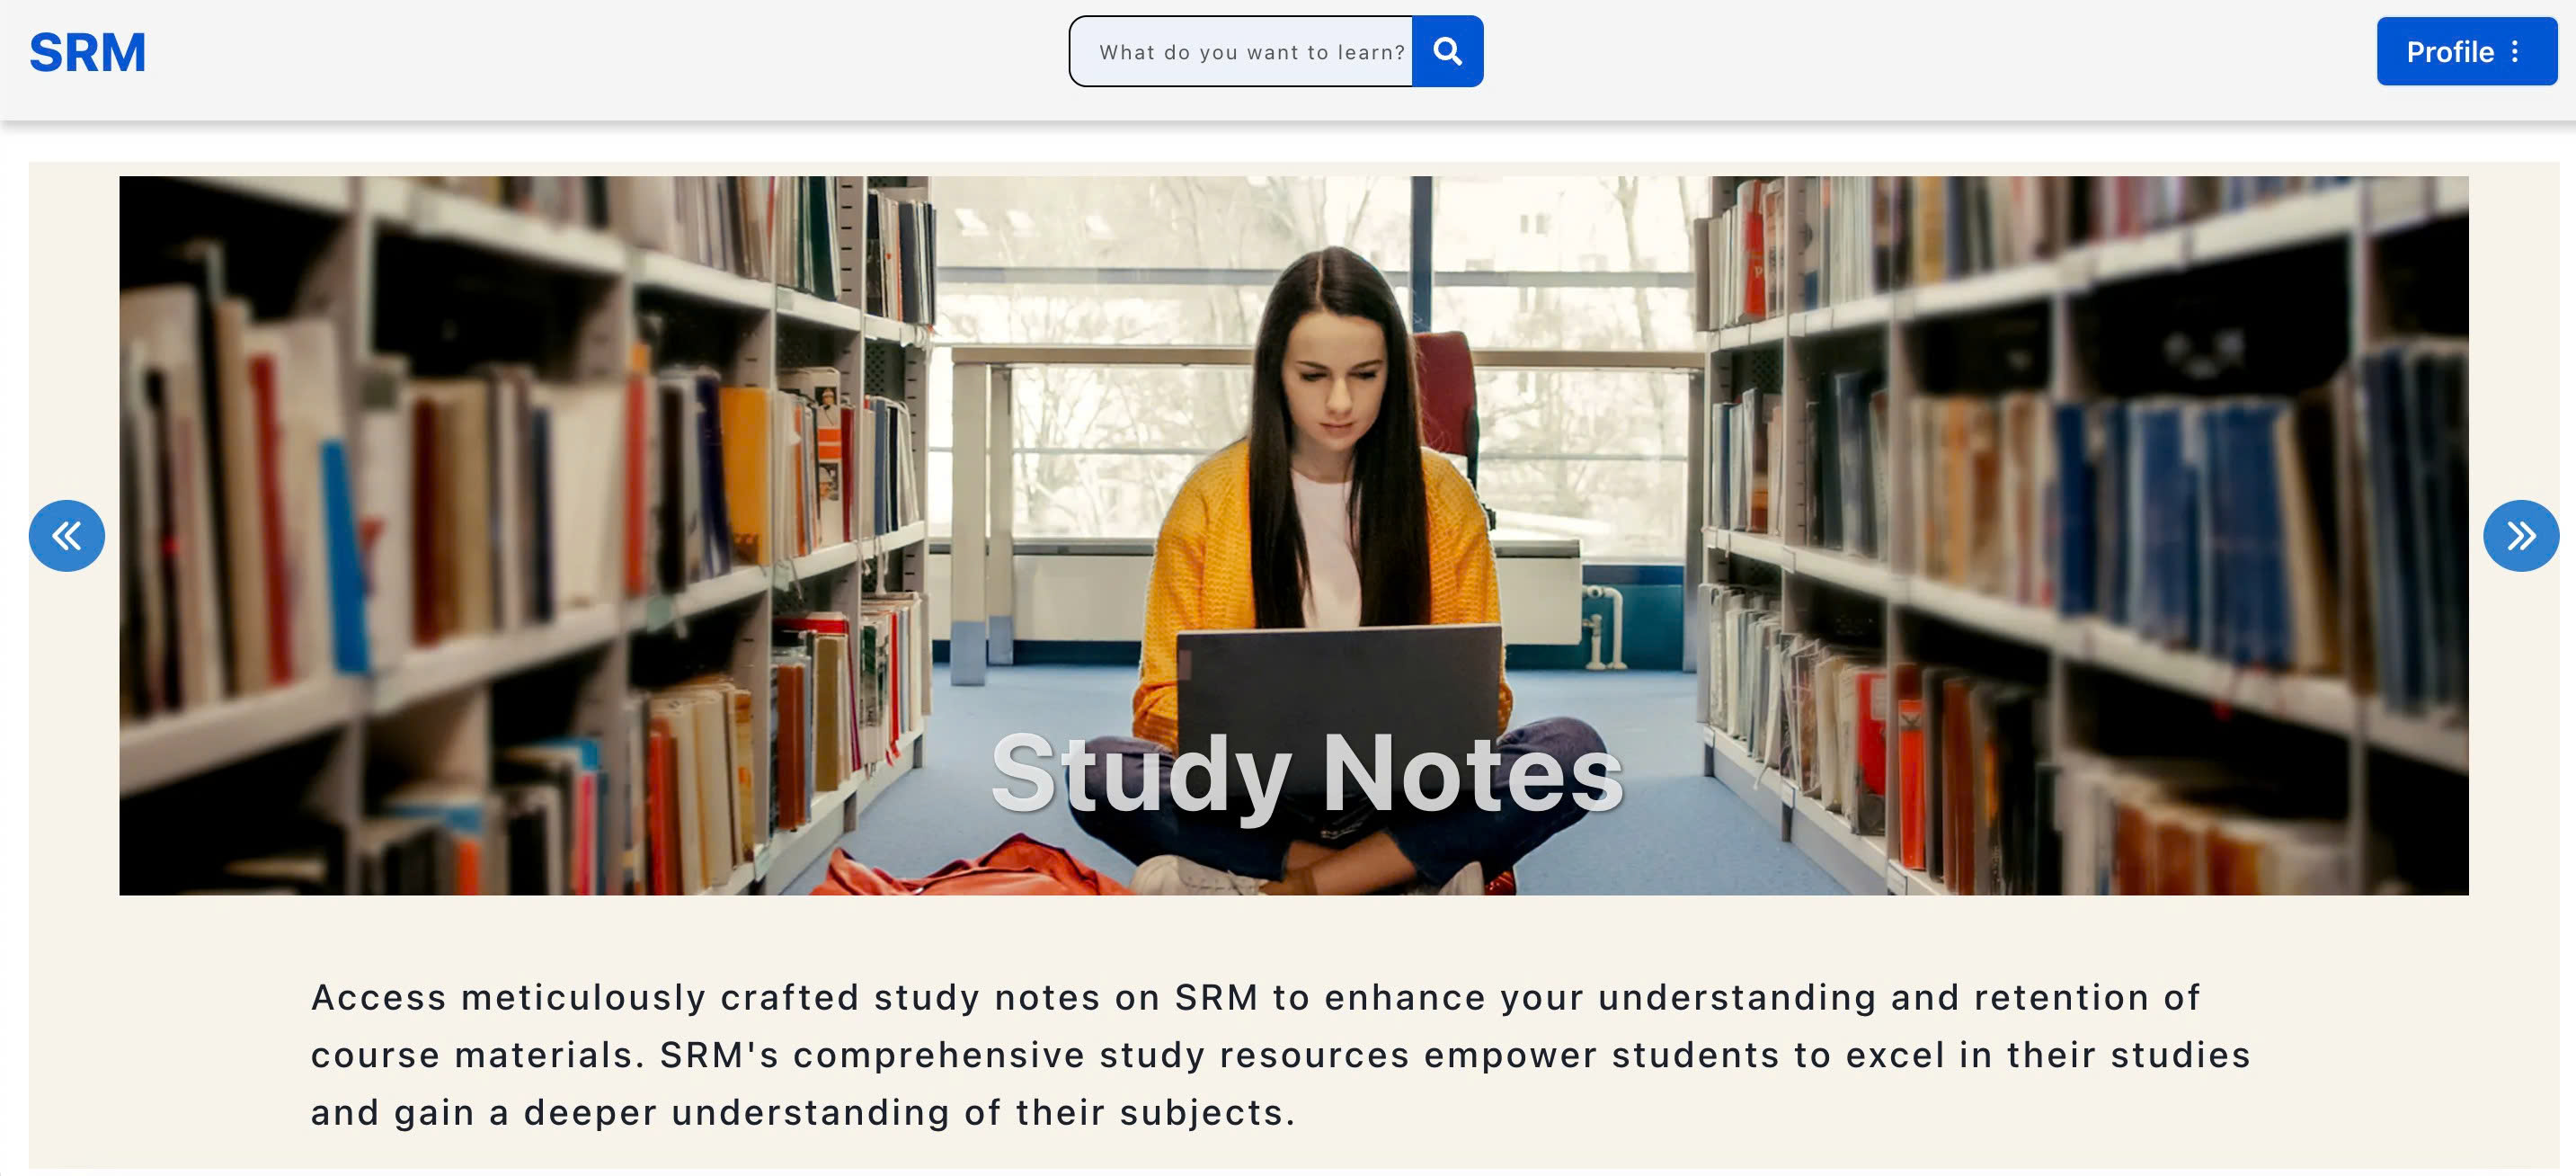
\includegraphics[width=0.8\textwidth]{figs/home_page.jpg}
\caption{Trang chủ (Landing Page)}
\label{fig:home}
\end{figure}

\begin{figure}[H]
\centering
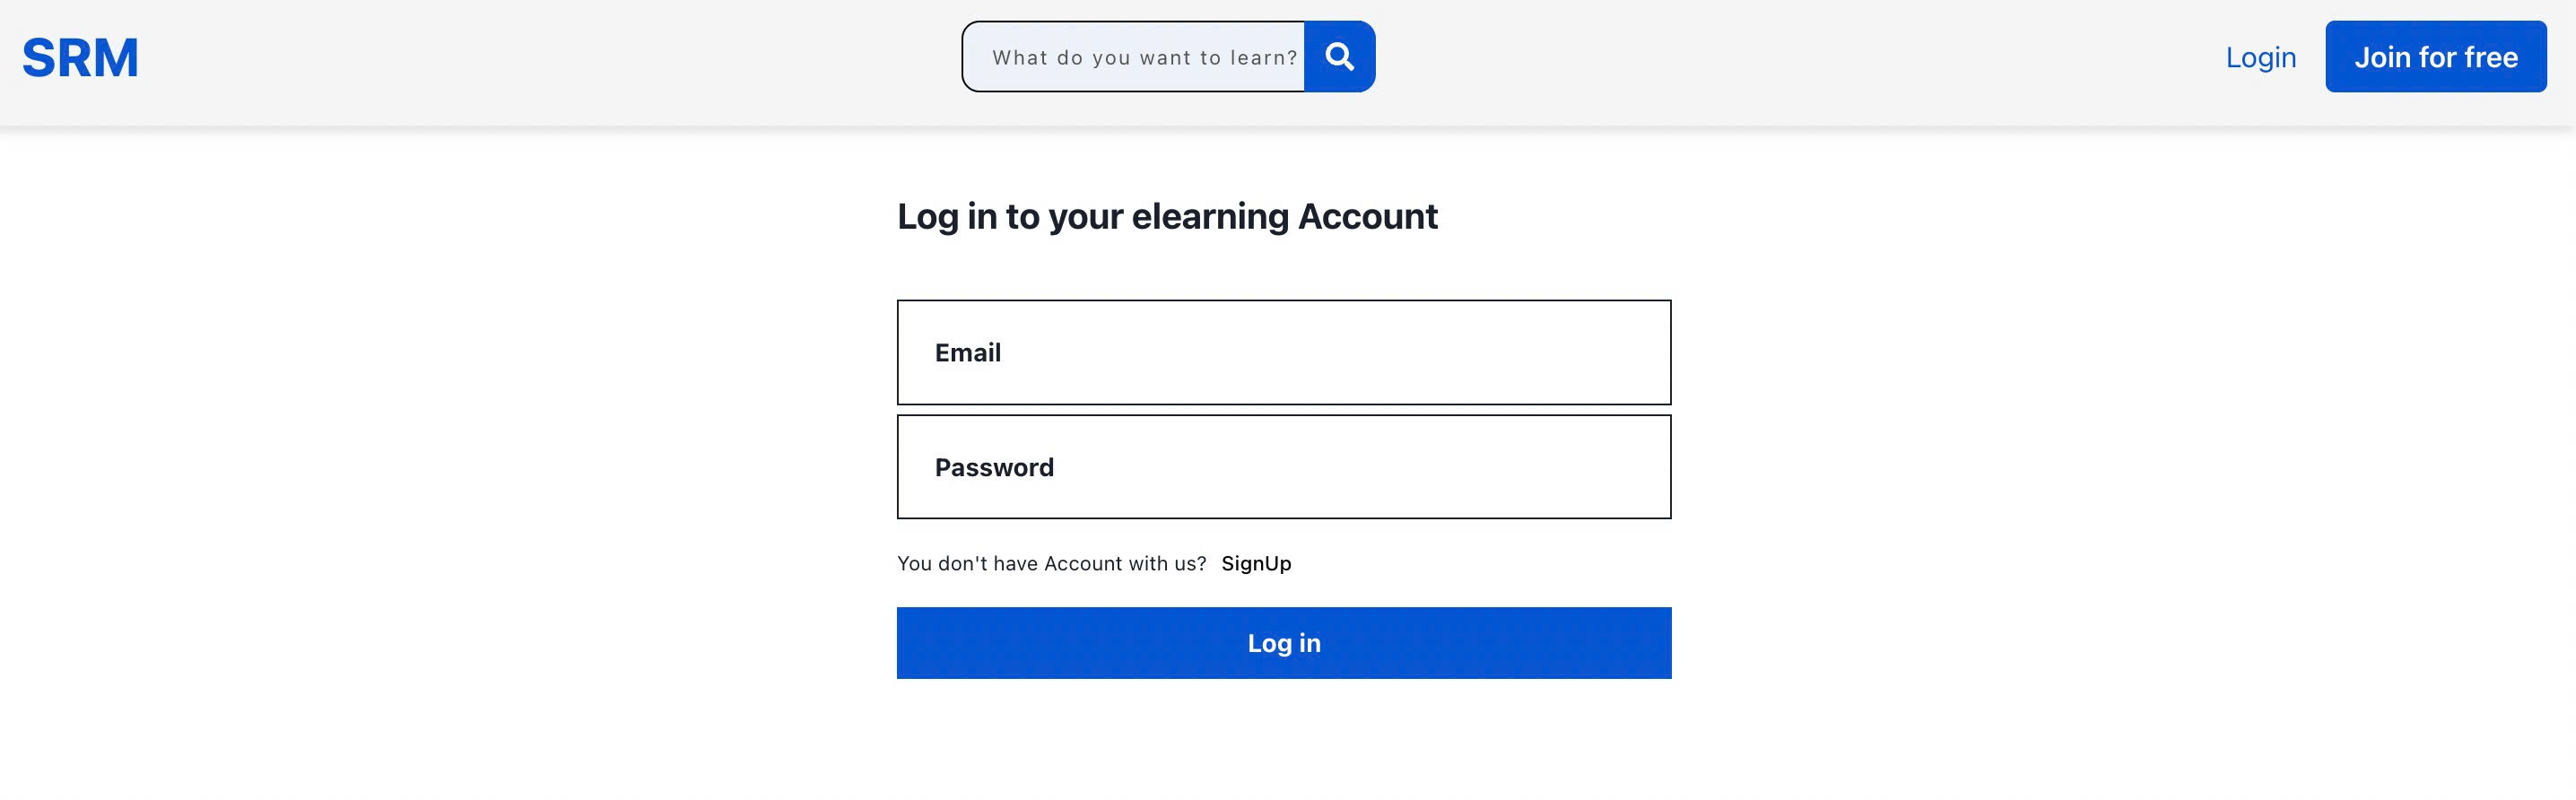
\includegraphics[width=0.8\textwidth]{figs/login_page.jpg}
\caption{Trang đăng nhập}
\label{fig:login}
\end{figure}

\begin{figure}[H]
\centering
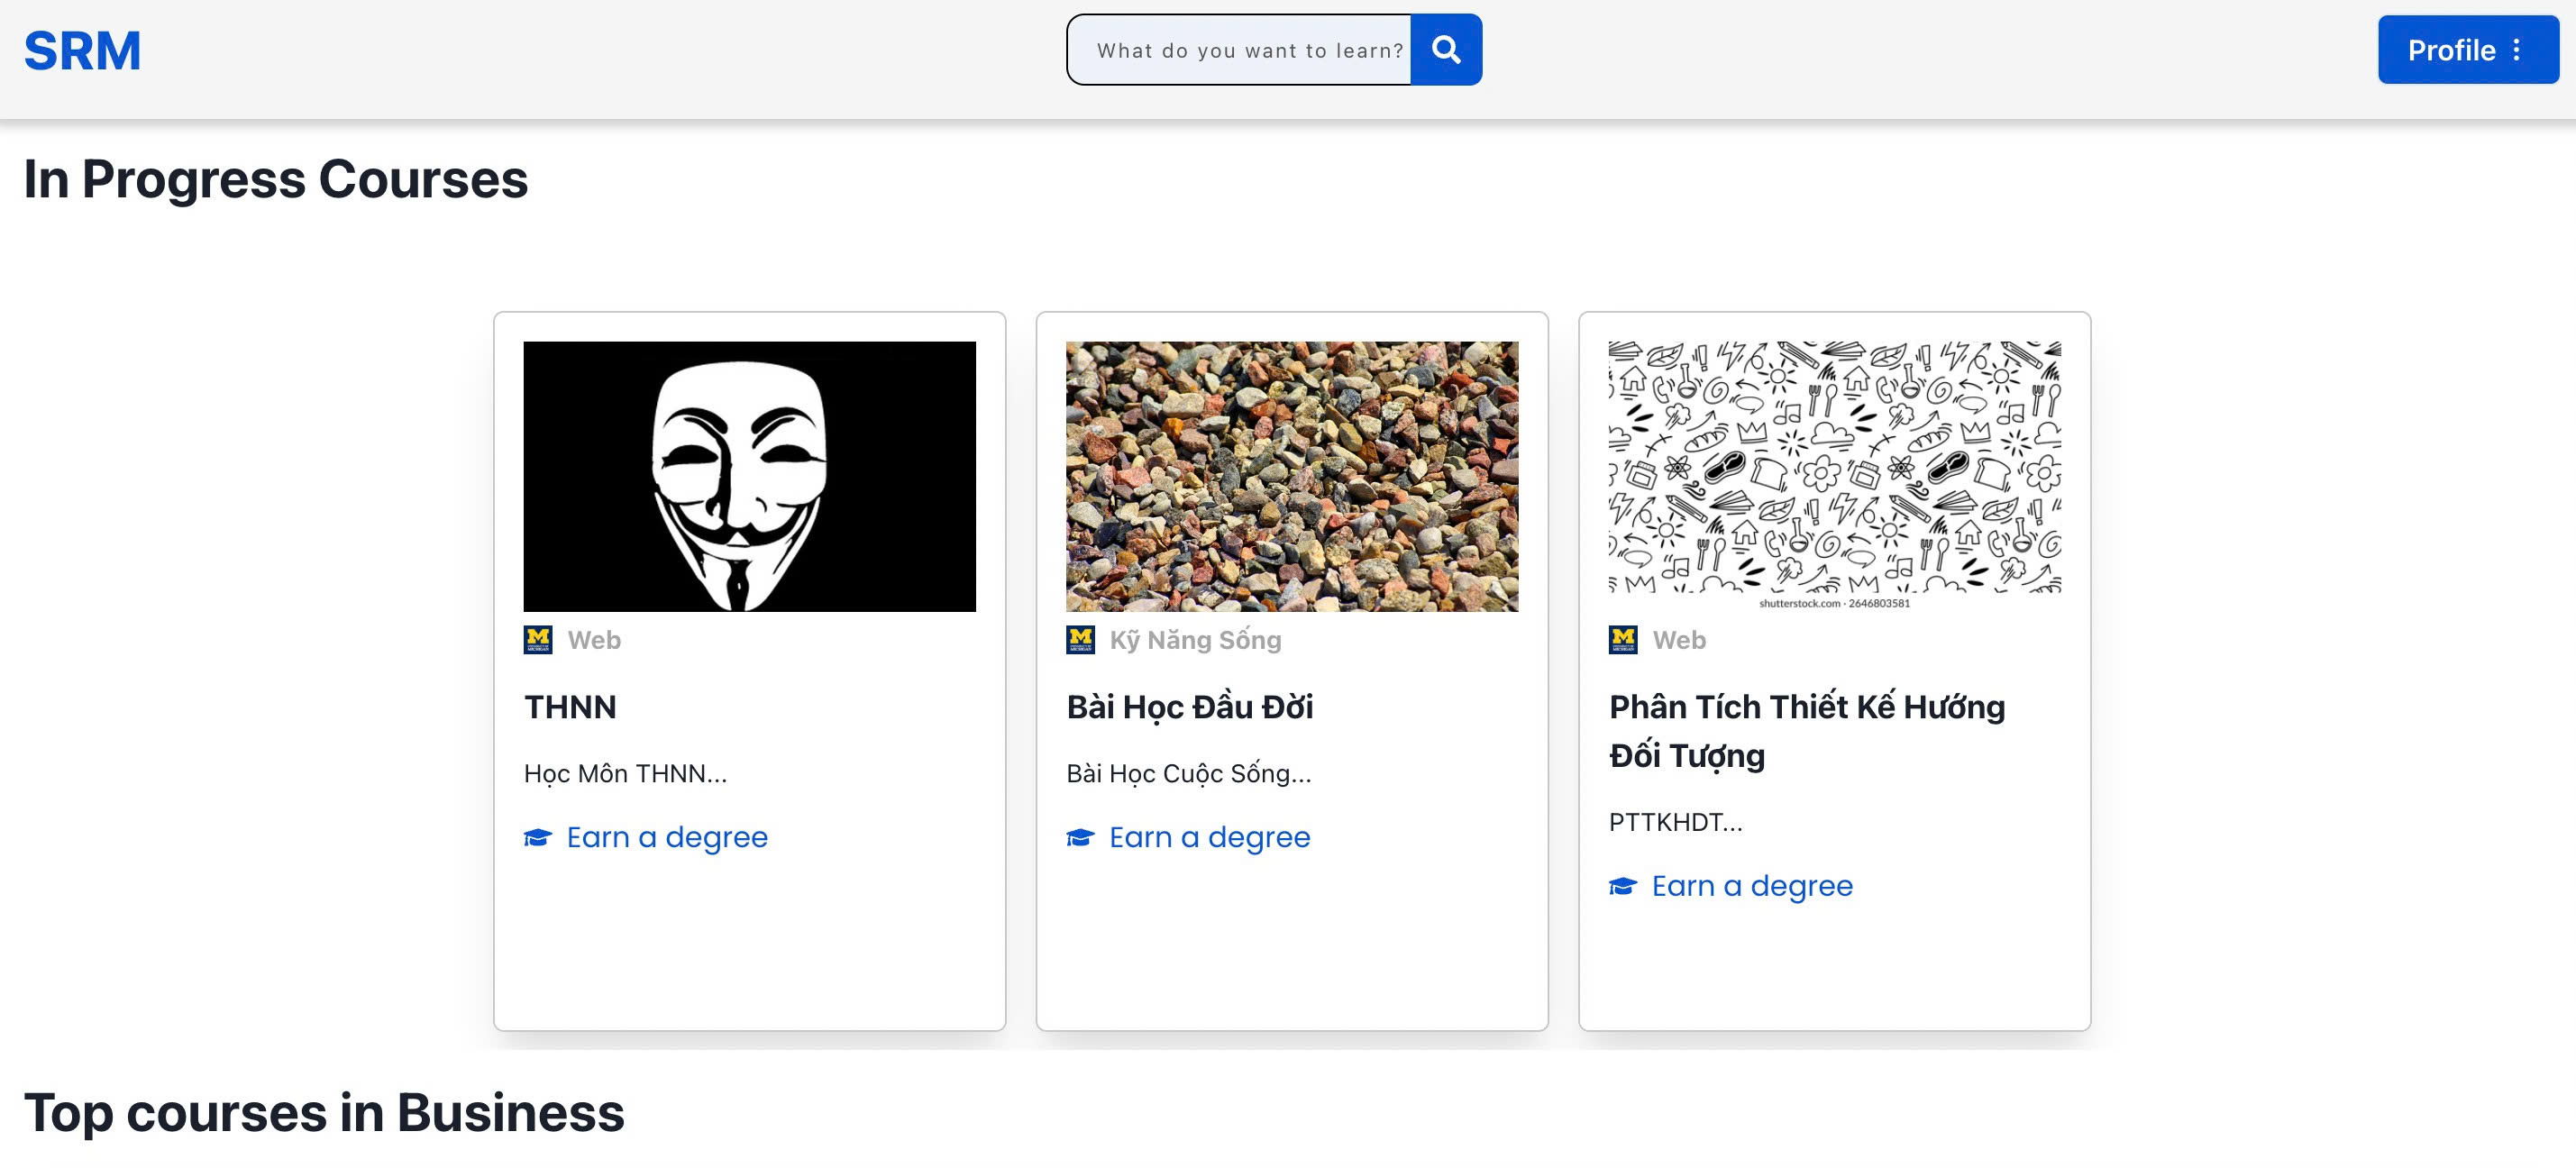
\includegraphics[width=0.8\textwidth]{figs/user_dashboard.jpg}
\caption{Dashboard của học viên}
\label{fig:user_dashboard}
\end{figure}

\begin{figure}[H]
\centering
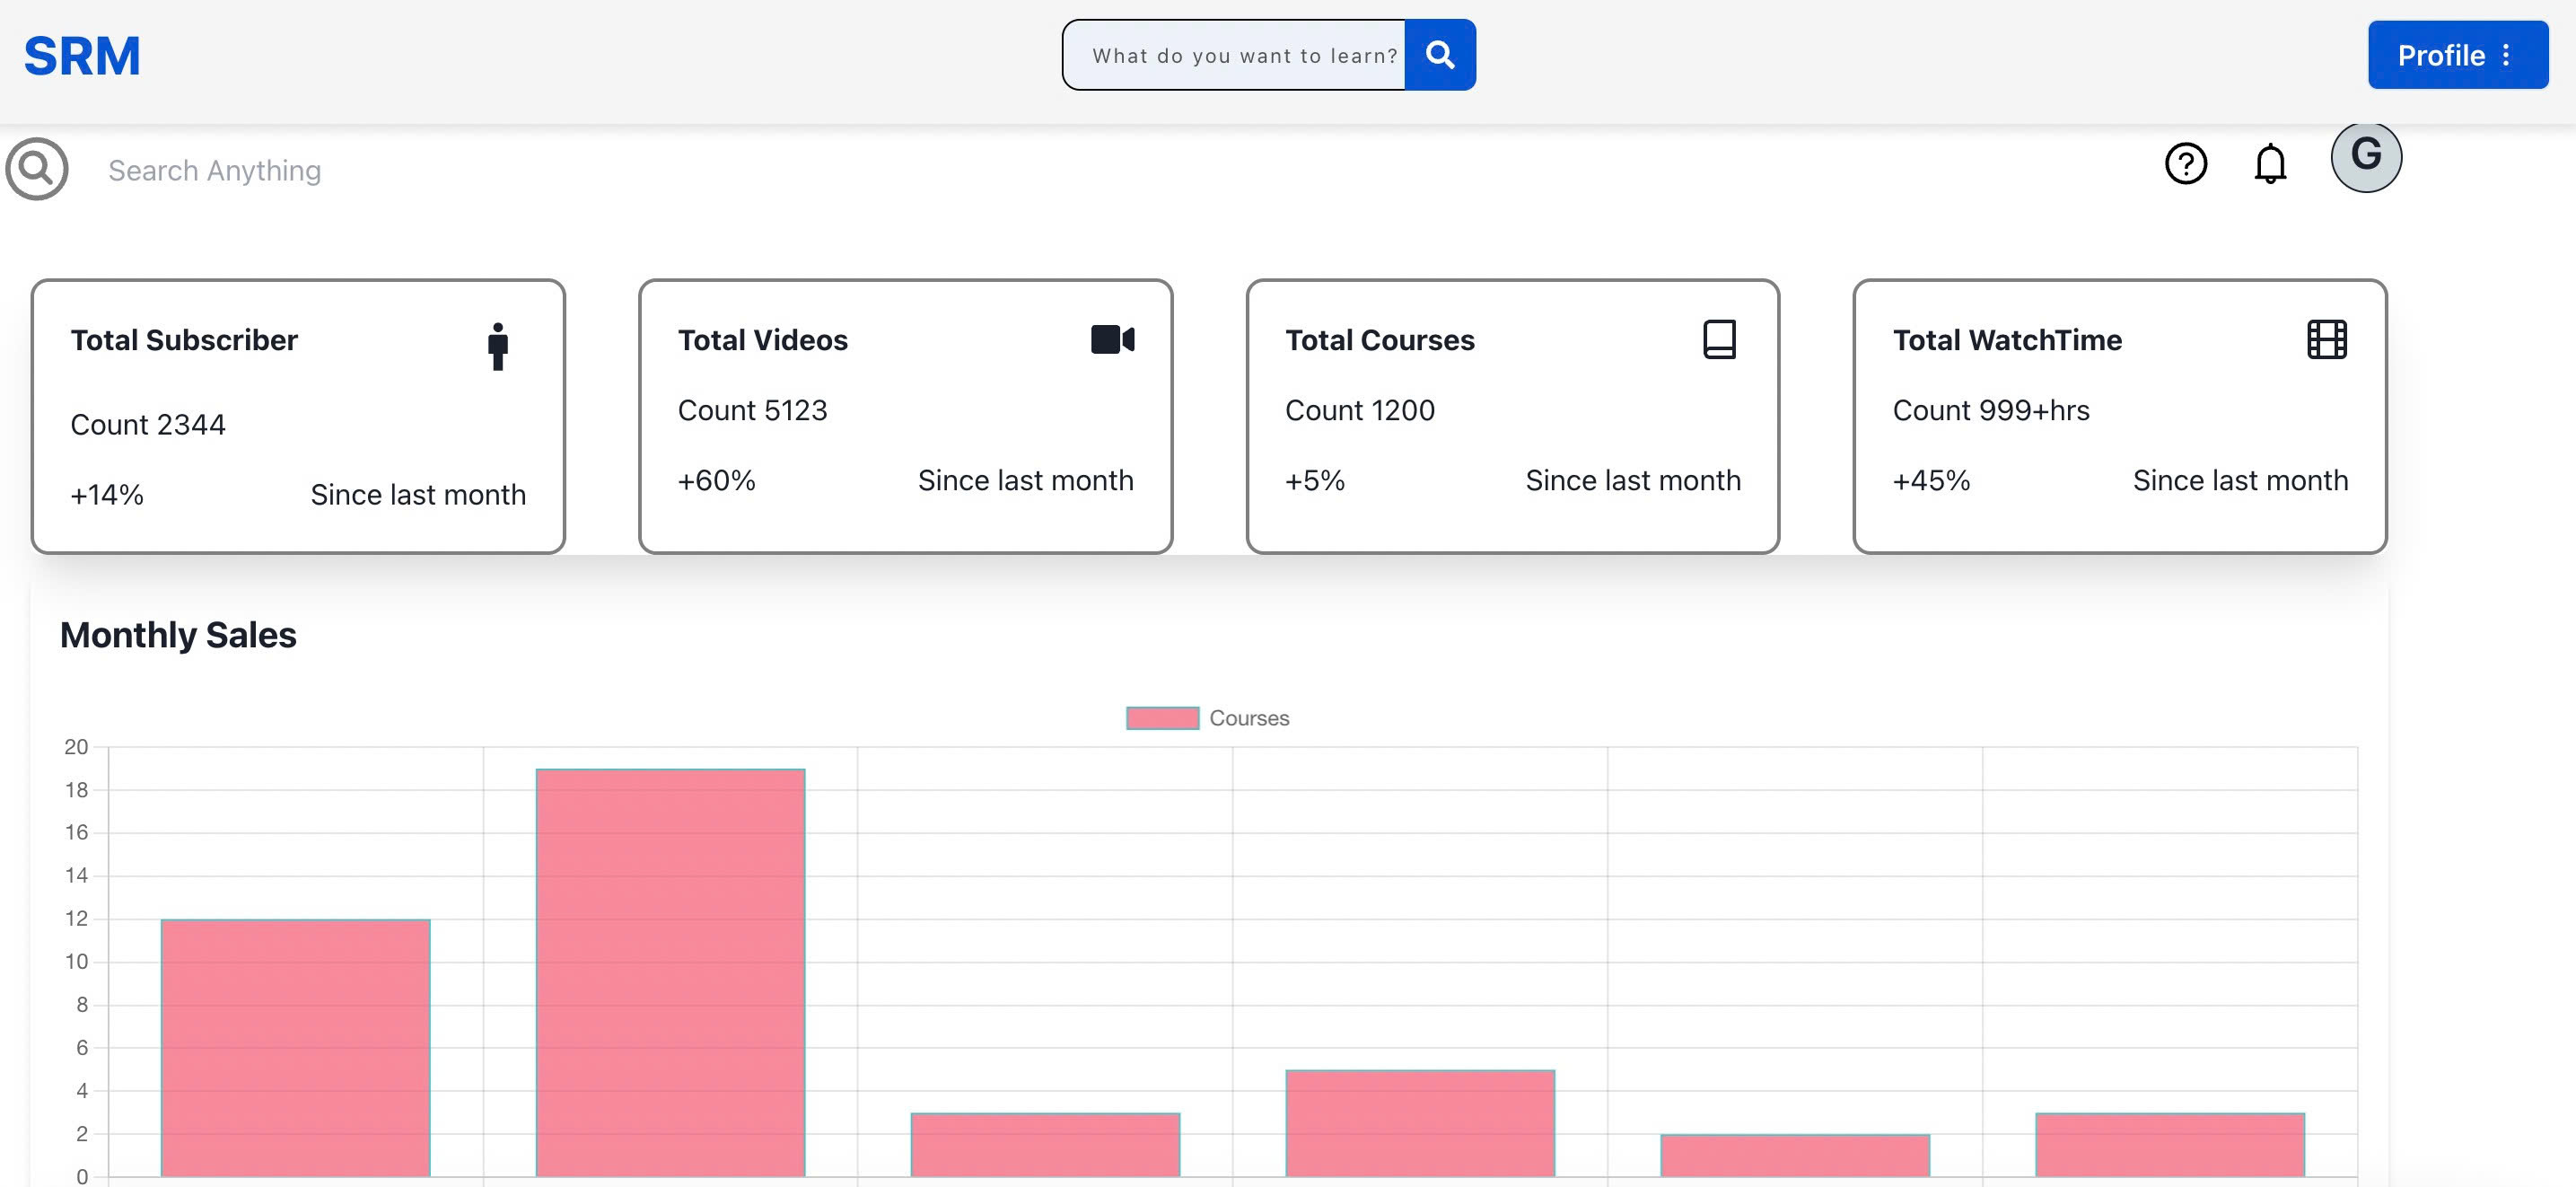
\includegraphics[width=0.8\textwidth]{figs/admin_dashboard.jpg}
\caption{Dashboard của quản trị viên}
\label{fig:admin_dashboard}
\end{figure}

\begin{figure}[H]
\centering
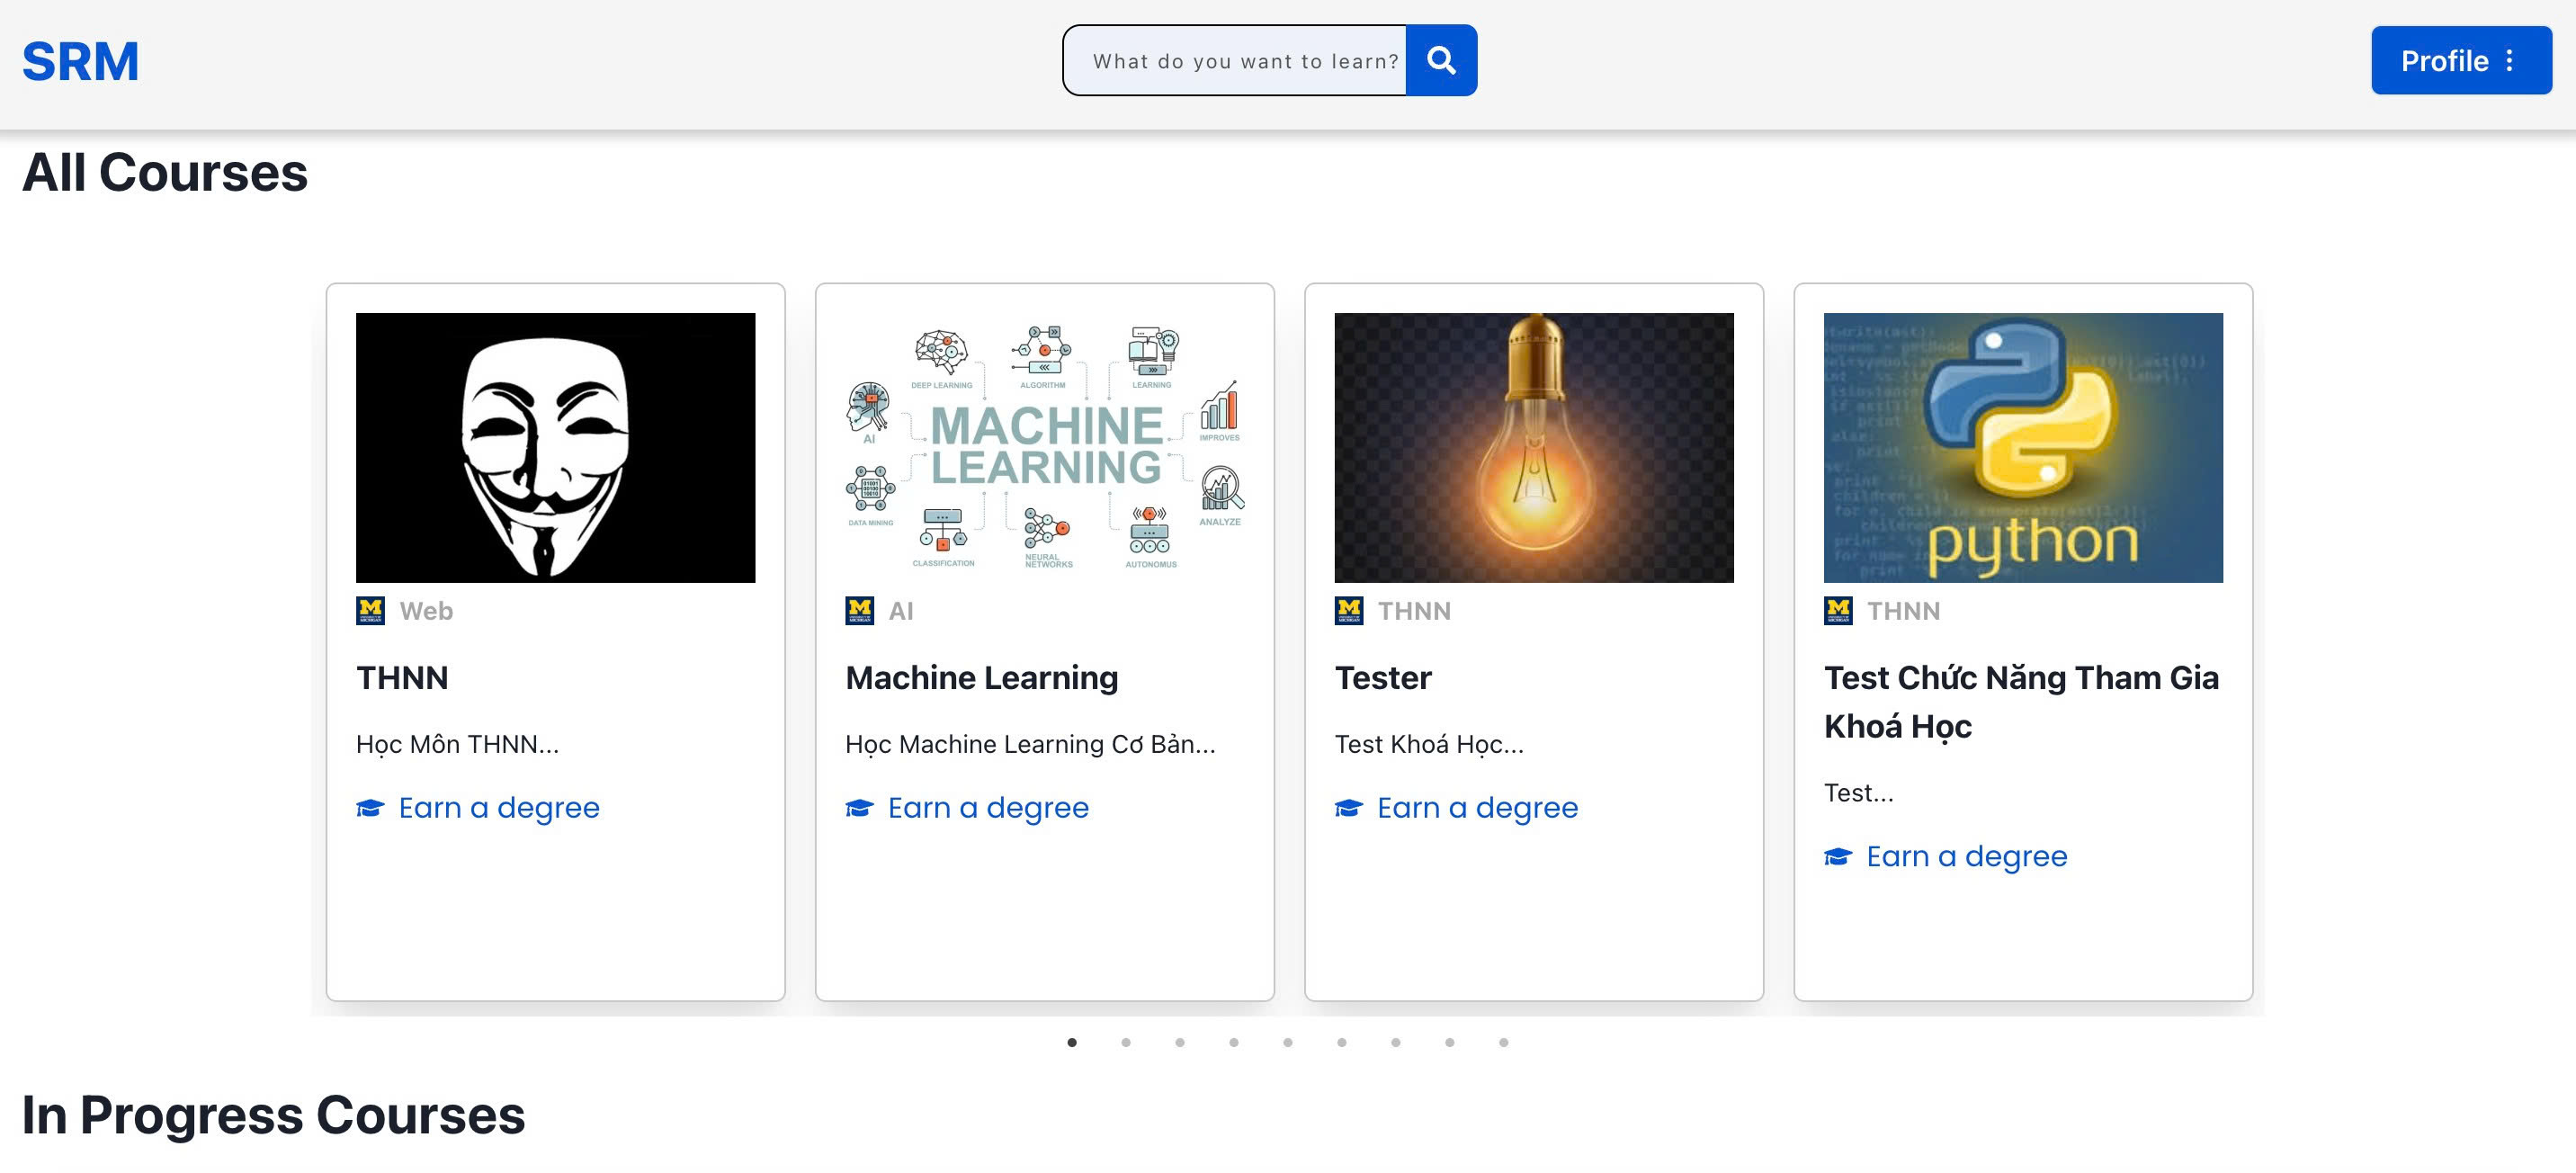
\includegraphics[width=0.8\textwidth]{figs/courses_overview.jpg}
\caption{Danh sách khóa học}
\label{fig:courses}
\end{figure}

(Ghi chú: Các ảnh chụp khác có thể tham khảo trong thư mục \texttt{screenshots})

\section{Thiết kế API}
Hệ thống xây dựng các RESTful API với cấu trúc chung: tiền tố `/api/v1`. Dưới đây là các endpoint chính.

\subsection{API Xác thực và Người dùng}
\begin{table}[H]
\centering
\caption{API Users \& Auth}
\begin{tabular}{|p{3cm}|p{2.5cm}|p{7cm}|}
\hline
\textbf{Endpoint} & \textbf{Method} & \textbf{Mô tả} \\ \hline
/api/auth/register & POST & Đăng ký tài khoản mới (student). \\ \hline
/api/auth/login & POST & Đăng nhập, trả về JWT token. \\ \hline
/api/auth/logout & POST & Đăng xuất (thêm token vào blacklist). \\ \hline
/api/users/profile & GET & Lấy thông tin cá nhân của user đang đăng nhập. \\ \hline
/api/users/profile & PUT & Cập nhật thông tin cá nhân. \\ \hline
/api/users & GET & (Admin) Lấy danh sách tất cả user. \\ \hline
/api/users/:id & PUT & (Admin) Cập nhật user (vai trò, khóa tài khoản). \\ \hline
/api/users/:id & DELETE & (Admin) Xóa user (nếu không có dữ liệu ràng buộc). \\ \hline
\end{tabular}
\end{table}

\subsection{API Quản lý khóa học}
\begin{table}[H]
\centering
\caption{API Courses}
\begin{tabular}{|p{3cm}|p{2.5cm}|p{7cm}|}
\hline
\textbf{Endpoint} & \textbf{Method} & \textbf{Mô tả} \\ \hline
/api/courses & GET & Lấy danh sách khóa học (có phân trang, lọc). \\ \hline
/api/courses/:id & GET & Lấy chi tiết khóa học. \\ \hline
/api/courses & POST & (Teacher/Admin) Tạo khóa học mới. \\ \hline
/api/courses/:id & PUT & (Teacher/Admin) Cập nhật khóa học. \\ \hline
/api/courses/:id & DELETE & (Teacher/Admin) Xóa khóa học. \\ \hline
/api/courses/:id/enroll & POST & (Student) Ghi danh vào khóa học. \\ \hline
/api/courses/my-courses & GET & (Student) Lấy khóa học đã ghi danh. \\ \hline
/api/courses/instructor & GET & (Teacher) Lấy khóa học do mình tạo. \\ \hline
\end{tabular}
\end{table}

\subsection{API Bài học và Quiz}
\begin{table}[H]
\centering
\caption{API Lessons \& Quizzes}
\begin{tabular}{|p{3cm}|p{2.5cm}|p{7cm}|}
\hline
\textbf{Endpoint} & \textbf{Method} & \textbf{Mô tả} \\ \hline
/api/courses/:courseId/lessons & GET & Lấy danh sách bài học của khóa học. \\ \hline
/api/lessons & POST & (Teacher) Thêm bài học mới. \\ \hline
/api/lessons/:id & PUT & (Teacher) Cập nhật bài học. \\ \hline
/api/lessons/:id & DELETE & (Teacher) Xóa bài học. \\ \hline
/api/lessons/:lessonId/quiz & GET & Lấy quiz của bài học. \\ \hline
/api/quizzes & POST & (Teacher) Tạo quiz mới. \\ \hline
/api/quizzes/:id & PUT & (Teacher) Sửa quiz. \\ \hline
/api/quizzes/:id/submit & POST & (Student) Nộp bài làm (tính điểm tự động). \\ \hline
/api/submissions/user & GET & (Student) Lấy kết quả các quiz đã làm. \\ \hline
\end{tabular}
\end{table}

\subsection{API Upload và Thống kê}
\begin{table}[H]
\centering
\caption{API Utils}
\begin{tabular}{|p{3cm}|p{2.5cm}|p{7cm}|}
\hline
\textbf{Endpoint} & \textbf{Method} & \textbf{Mô tả} \\ \hline
/api/upload & POST & Upload file (hình ảnh, video) lên Cloudinary. \\ \hline
/api/admin/stats & GET & (Admin) Lấy thống kê tổng quan (số user, course, doanh thu). \\ \hline
/api/admin/stats/export & GET & (Admin) Xuất báo cáo Excel. \\ \hline
\end{tabular}
\end{table}

\section{Kết luận chương}
Chương 3 hoàn thành thiết kế cơ sở dữ liệu với 6 collection, các ràng buộc toàn vẹn; thiết kế kiến trúc 3 lớp; thiết kế giao diện trực quan; và thiết kế RESTful API chi tiết. Đây là cơ sở vững chắc để chuyển sang cài đặt và kiểm thử ở các chương tiếp theo.
